\documentclass[../report.tex]{subfiles}
\graphicspath{{\subfix{../image/}}}

\begin{document}
\subsection{Research and Evaluation for Loadcell-Interfacing}

\subsection{Choice of loadcells}

One of the functionalities of the forklift is measuring the weight lifted.
This serves the purpose of ensuring safe operations not only for customers, 
but also preventing the forklift from tilting or damaging itself in one way or the other.

In accordance to the set requirements, the forklift should at least lift 3.5kg.
Hence, the loadcells should be able to withstand this weight. 
Next to buying new loadcells, one possible option is to take the loadcells
out of a kitchen weight rated for that weight. This is beneficial in serveral aspects.
Not only does it give a insight into reverse engineering, but also provides beneficial
insight in classifying unknown sensor characteristics. Furthermore, it does not 
stress the budget. 

\quad
Insert picture of loadcells here.

A kitchen scale rated for max. 5kg was bought. The four loadcells of this scale were taken to the lab and
their behavior was evaluated. 

\quad

Conclusion: The loadcells suit the application. They can not only withstand the
required stress-requirements, but also work reliable. Moreover, they fulfill the 
space requirements for the "small-scale" fork. Furthermore, they bring a considerable
learning effect with them.

\quad

The next engineering challenge is interfacing these loadcells.
These loadcells include two variable resistances. One of them increases
with stress the other one decreases with stress. 

\quad

Interfacing bears serveral challenges:

\begin{itemize}

  \item Output of interface must be compatible with ADC range of microcontroller.
  \item Current through loadcells must be limited.
  \item Output needs to be amplified.

\end{itemize}

\subsection{Available Options}

In this section the available options to overcome these challenges are discussed.

\begin{itemize}

  \item HX711 Interface Module and load-cell
  \item Wheatstone bridge - in different configuration
  \begin{itemize}
    \item With constant current source
    \item Without constant current source
  \end{itemize}

\end{itemize}

\subsubsection{HX711 Interface Module and load-cell}

A Load Cell serves as a sensor that transforms applied force, encompassing pressure, rotational force, compression, or tension, into quantifiable electrical signals.
The load cell generates an output in millivolt range; therefore, it is essential to magnify this signal into a higher-level amplitude and subsequently convert it into a digital format for further processing.
To accomplish this task, the HX711 interface module could be used. This was recommended by a professor. This module serves to amplify the load cell's low-voltage output and transmit it to the microcontroller for weight calculation. 
The illustration below depicts the HX711 interface module.


\begin{figure}[H]
    \centering
    \begin{subfigure}[b]{0.4\linewidth}
      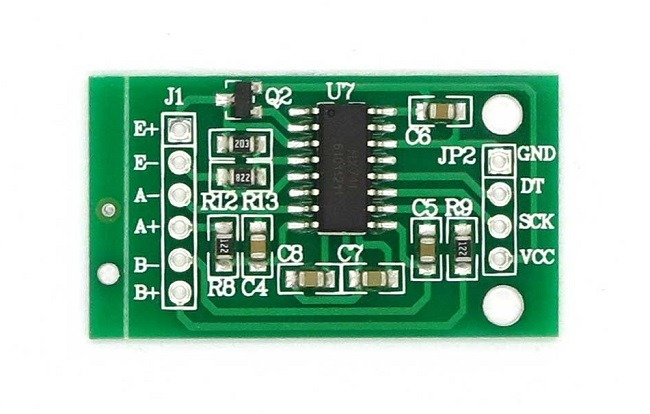
\includegraphics[width=\linewidth]{image/HX711-Weighing-Sensor-Dual-Channel-24-Bit-Precision-A-D-Module-Pressure-Sensor_1.jpg}
      \caption{HX711 Interface Module }
    \end{subfigure}
    \begin{subfigure}[b]{0.4\linewidth}
      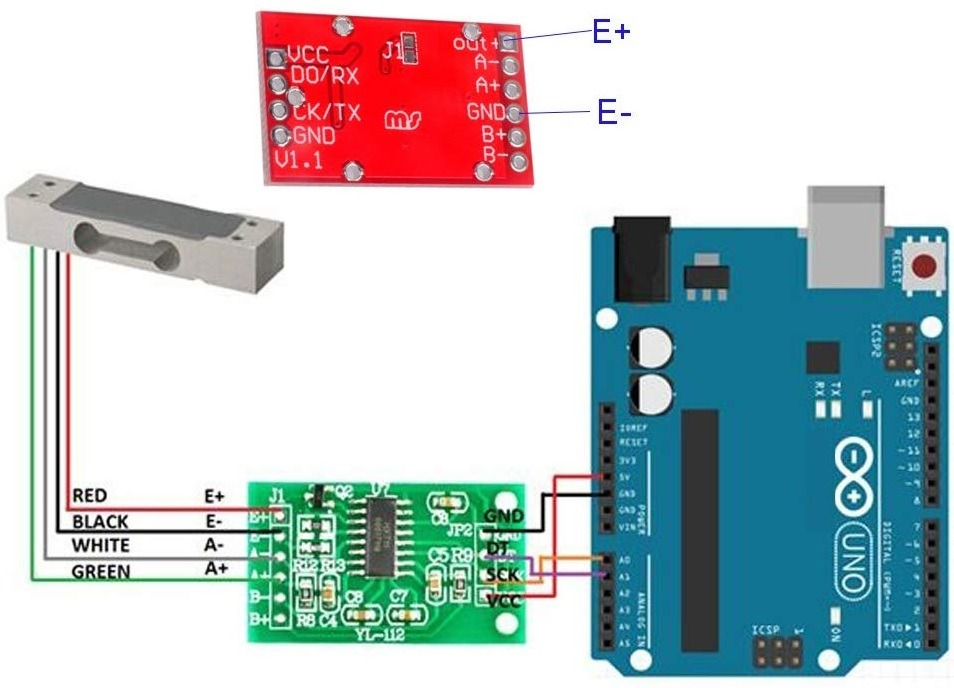
\includegraphics[width=\linewidth]{image/hx711-red.jpg}
      \caption{HX711 Interface Module and Load cell using Arduino}
    \end{subfigure}
    
    
  \end{figure}
  
\end{document}